\documentclass[tikz,border=2pt]{standalone}
\usepackage{amsmath}
\usetikzlibrary{arrows.meta,calc}
\begin{document}
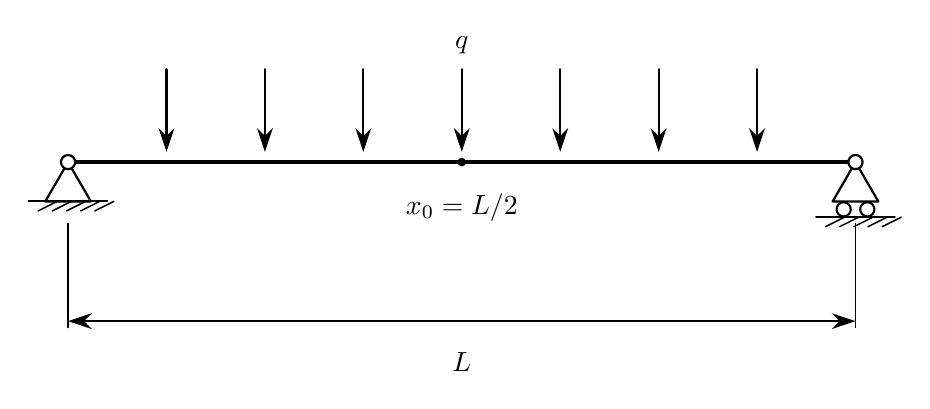
\begin{tikzpicture}[
  line cap=round,
  line join=round,
  every node/.style={font=\normalsize}
]
  \def\L{10.0}
  \def\yb{0.0}
  \def\supportdrop{0.68}

  % Beam axis.
  \draw[black, line width=1.15pt] (0,\yb) -- (\L,\yb);

  % Symmetric distributed load markers.
  \foreach \x in {1.25,2.50,3.75,5.00,6.25,7.50,8.75} {
    \draw[black, -{Stealth[length=3.0mm,width=2.0mm]}, line width=0.75pt]
      (\x,1.18) -- (\x,0.13);
  }
  \node at (5.00,1.48) {$q$};

  % Midspan response point and label.
  \filldraw[black] (5.00,\yb) circle (1.35pt);
  \node[below=8pt] at (5.00,\yb) {$x_0=L/2$};

  % Left pin support.
  \draw[black, line width=0.8pt] (-0.29,-0.50) -- (0,\yb) -- (0.29,-0.50) -- cycle;
  \draw[black, line width=0.75pt] (-0.50,-0.50) -- (0.50,-0.50);
  \foreach \x in {-0.38,-0.20,-0.02,0.16,0.34} {
    \draw[black, line width=0.55pt] (\x,-0.62) -- (\x+0.24,-0.50);
  }
  \draw[fill=white, draw=black, line width=0.8pt] (0,\yb) circle (0.09);

  % Right roller support.
  \draw[black, line width=0.8pt] (\L-0.29,-0.50) -- (\L,\yb) -- (\L+0.29,-0.50) -- cycle;
  \draw[black, line width=0.75pt] (\L-0.50,-0.70) -- (\L+0.50,-0.70);
  \draw[black, line width=0.75pt] (\L-0.15,-0.60) circle (0.09);
  \draw[black, line width=0.75pt] (\L+0.15,-0.60) circle (0.09);
  \foreach \x in {\L-0.38,\L-0.20,\L-0.02,\L+0.16,\L+0.34} {
    \draw[black, line width=0.55pt] (\x,-0.82) -- (\x+0.24,-0.70);
  }
  \draw[fill=white, draw=black, line width=0.8pt] (\L,\yb) circle (0.09);

  % Dimension line.
  \draw[black, line width=0.55pt] (0,-0.78) -- (0,-2.10);
  \draw[black, line width=0.55pt] (\L,-0.78) -- (\L,-2.10);
  \draw[black, {Stealth[length=3mm,width=2mm]}-{Stealth[length=3mm,width=2mm]}, line width=0.75pt]
    (0,-2.02) -- (\L,-2.02);
  \node[below=8pt] at (5.00,-2.02) {$L$};
\end{tikzpicture}
\end{document}
